
%(BEGIN_QUESTION)
% Copyright 2010, Tony R. Kuphaldt, released under the Creative Commons Attribution License (v 1.0)
% This means you may do almost anything with this work of mine, so long as you give me proper credit

Determine the amount of air pressure applied to this water manometer, answering both in units of kPa and units of inches water column.  Assume the scale is calibrated in {\it inches}:

$$\includegraphics[width=15.5cm]{i03711x01.eps}$$

$P$ = \underbar{\hskip 50pt} kPa

\vskip 10pt

$P$ = \underbar{\hskip 50pt} inches water column

\underbar{file i03711}
%(END_QUESTION)





%(BEGIN_ANSWER)

\noindent
5 points each answer:

\vskip 10pt

$P$ = \underbar{\bf 1.121} kPa

\vskip 10pt

$P$ = \underbar{\bf 4.5} inches water column


%(END_ANSWER)





%(BEGIN_NOTES)

{\bf This question is intended for exams only and not worksheets!}.

%(END_NOTES)


